\section{Cemetery Plot Lists}

\setlength{\parindent}{0cm}

See also the O'Brien ``virtual cemetery'' on Find a Grave: \url{https://www.findagrave.com/virtual-cemetery/1084932}\index{Find a Grave}\\
\\
For more information on Catholic Mt.\ Auburn Cemetery, see Bill McEvoy's book and the Historical Society of Watertown website: \url{http://historicalsocietyofwatertownma.org/HSW/index.php?option=com_content&view=article&id=124&Itemid=64}
\\
Women's maiden names and corrected names appear in brackets.

\begin{table}[ht]
	\centering
		\caption{North Cambridge Catholic Cemetery\index{North Cambridge Catholic Cemetery}\cite{DianaBerberenaLetter1} \\
		Cambridge, Middlesex County, Massachusetts\index{Massachusetts!Cambridge}
		Range 17, Grave 124 West (no marker found)}
	\begin{tabular}{|l|l|}
		\hline
		\textbf{Name} & \textbf{Death/Burial Date} \\
		\hline
	Mary Ann O'Brien\index{O'Brien!Mary Ann\textsuperscript{3} (1852--1852)} & (d) 25 Nov 1852 \\
	\hline
	William O'Brien\index{O'Brien!William\textsuperscript{1}} & (b) 30 Dec 1856 \\
	\hline
	Ellen O'Brien\index{O'Brien!Ellen\textsuperscript{3} (1853--1857)} & (d) 10 Mar 1857 \\
	\hline
	\end{tabular}
\end{table}

\begin{table}[ht]
	\centering
	\caption{Holy Cross Cemetery\index{Holy Cross Cemetery}\cite{HolyCrossPlot} \\
		Malden, Middlesex County, Massachusetts\index{Massachusetts!Malden}
		17 North Monument Path, Graves 32--34 East}
	\begin{tabular}{|l|l|}
		\hline
		\textbf{Name} & \textbf{Burial Date} \\
	\hline
	Edward O'Brien\index{O'Brien!Edward/Edmund\textsuperscript{2}} & 26 Aug 1881 \\
	\hline
	Edward J.\ O'Brien\index{O'Brien!Edward\textsuperscript{3} (1861--1884)} & 10 Jan 1884 \\
	\hline
	Ann Dailey [O'Brien]\index{O'Brien!Ann\textsuperscript{2}}\index{Dailey!Ann\textsuperscript{2} (O'Brien)} & 25 Sep 1898 \\
	\hline
	Mary Ward [O'Brien]\index{O'Brien!Mary\textsuperscript{2}}\index{Ward!Mary\textsuperscript{2} (O'Brien)} & 26 Mar 1908 \\
	\hline
	Hannah Flynn [Ward]\index{Ward!Hannah/Hanora\textsuperscript{3}}\index{Flynn!Hannah/Hanora\textsuperscript{3} (Ward)} & 12 Jan 1919 \\
	\hline
	Margaret A.\ O'Brien\index{O'Brien!Margaret A.\textsuperscript{3} (1859--1933)} & 08 Nov 1933 \\
	\hline
	Annie M.\ O'Brien\index{O'Brien!Ann\textsuperscript{3}} & 27 May 1937 \\
	\hline
	Anna Gertrude Duckworth\index{Duckworth!Anna Gertrude} & 29 Dec 1987 \\
	\hline
	Arthur R.\ Duckworth\index{Duckworth!Arthur R.} & 08 Mar 1994 \\
	\hline
	Jeanne A.\ Benson\index{Benson!Jeanne A.} & 08 Apr 2010 \\
	\hline
	Robert K.\ Benson\index{Benson!Robert K.} & 08 Aug 2014 \\
	\hline
	\end{tabular}
\end{table}

\begin{figure}
	\centering
	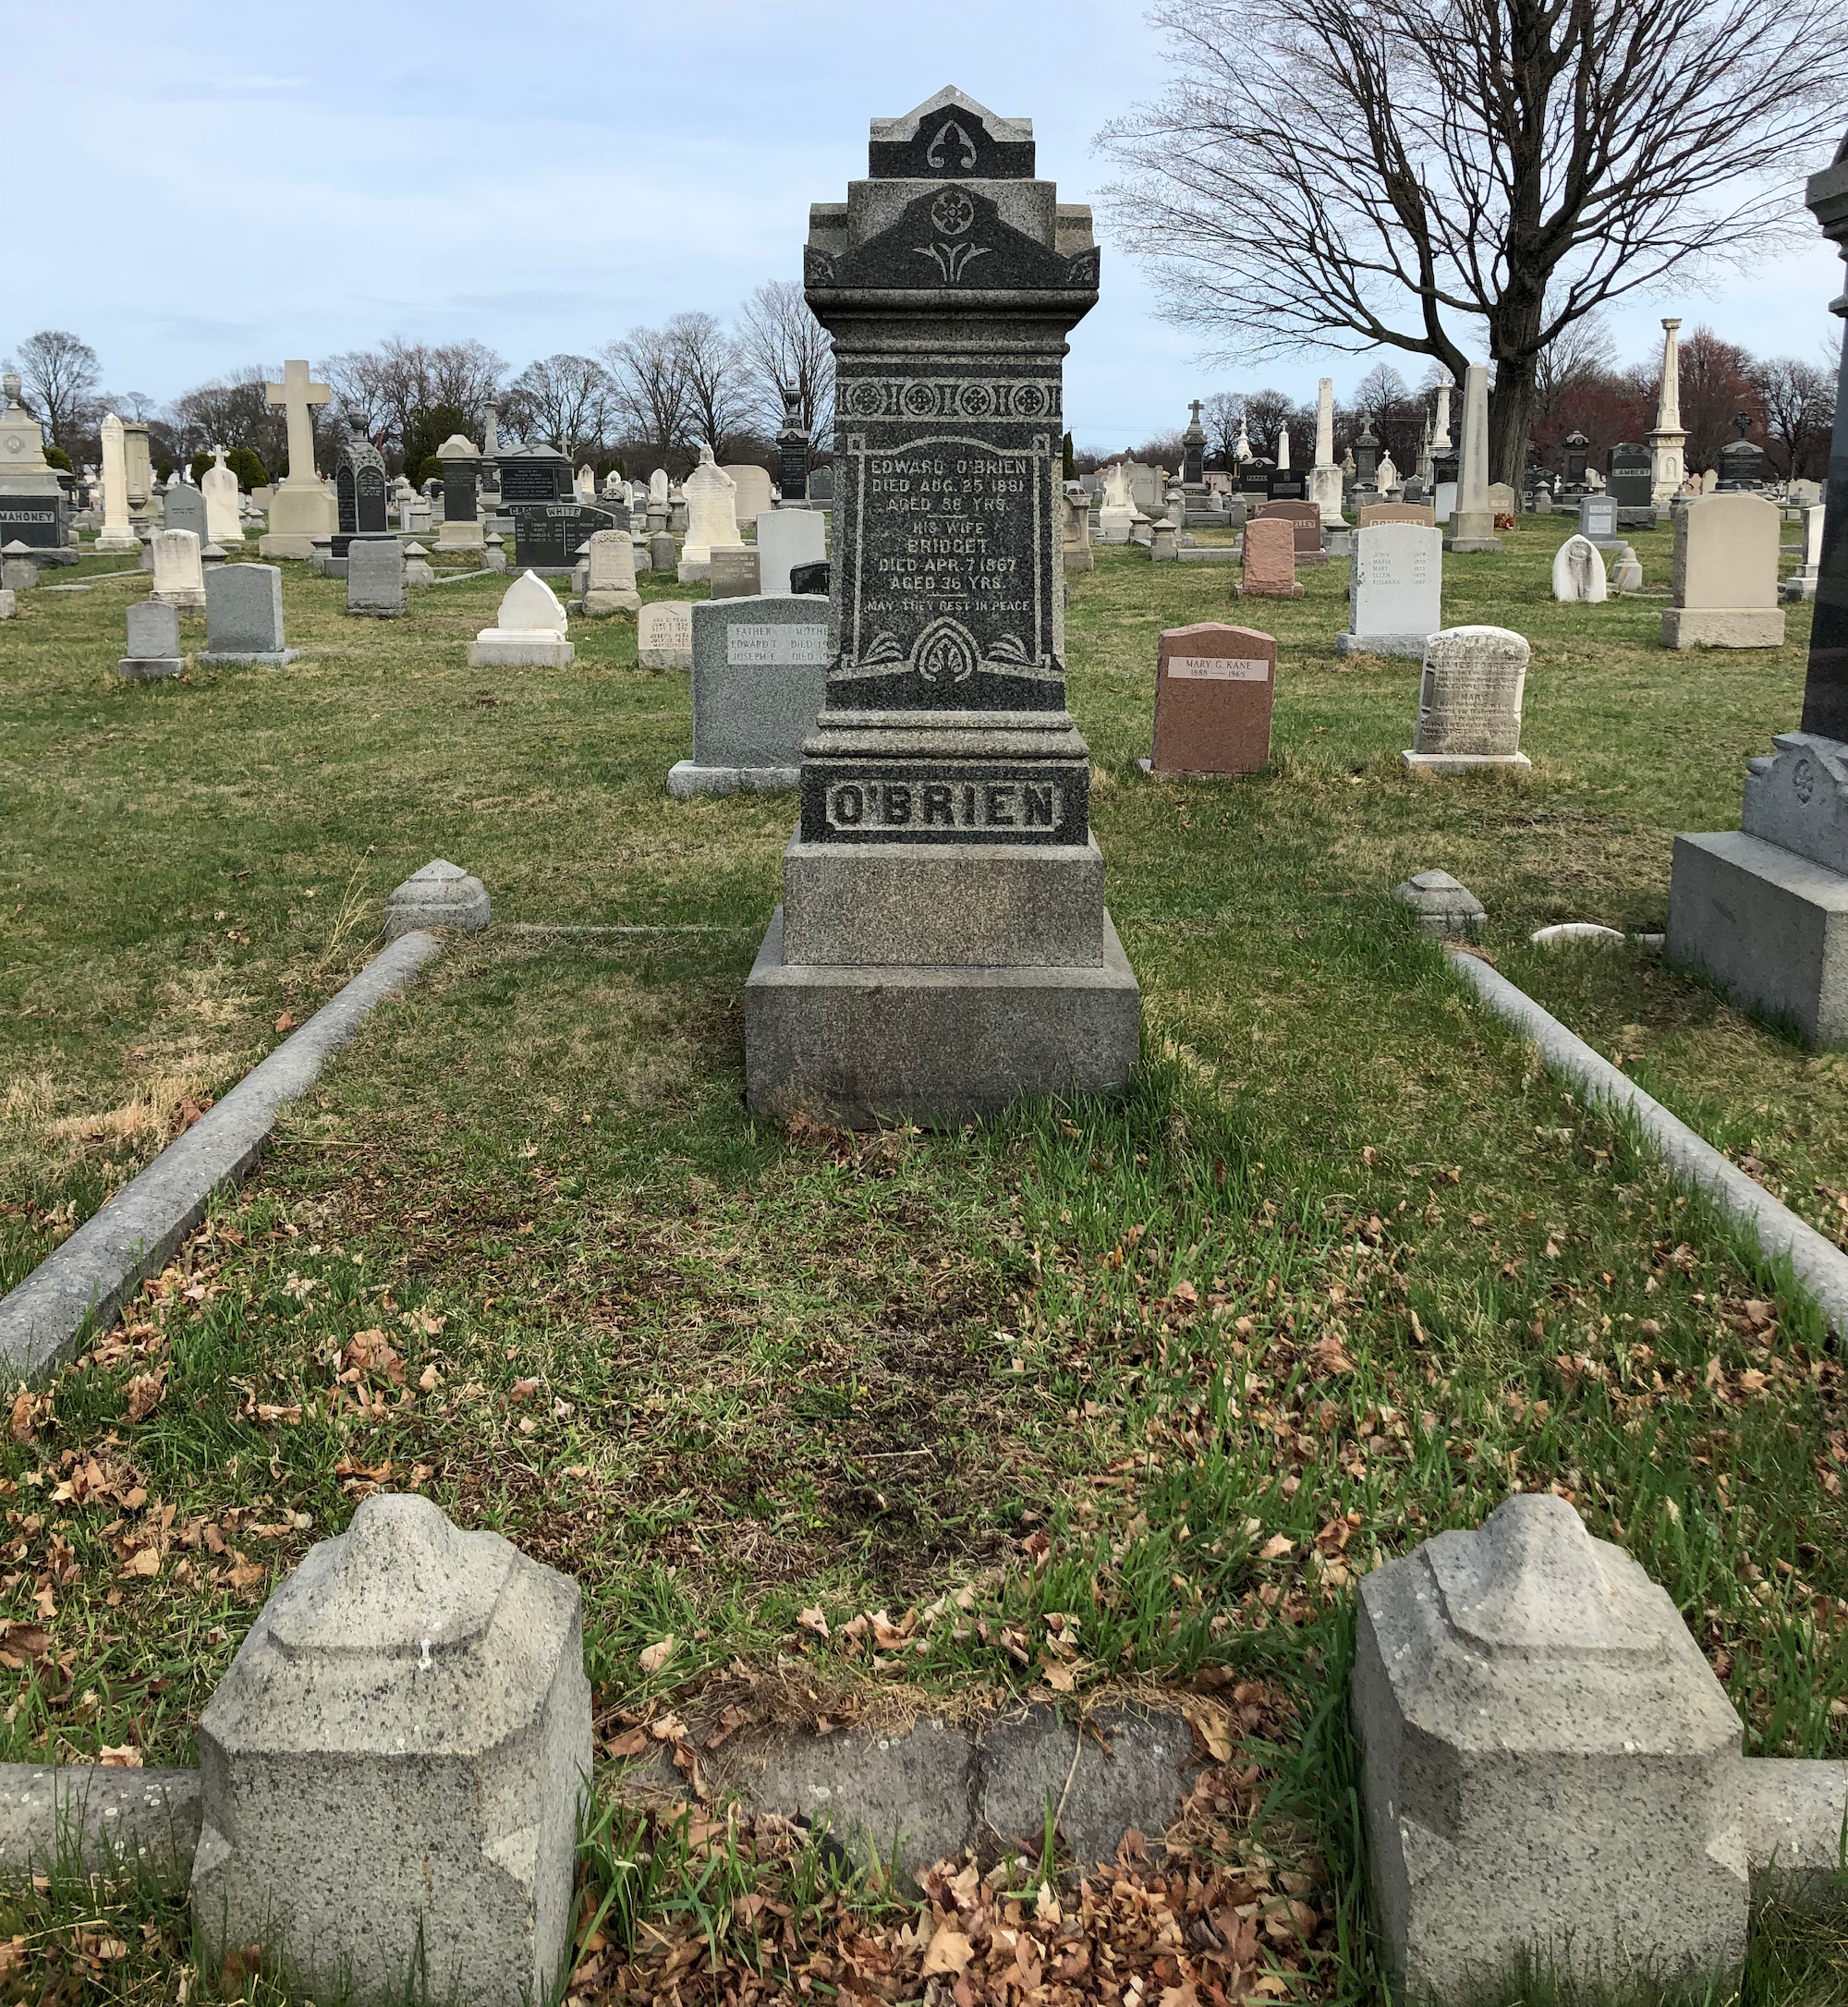
\includegraphics[width=\textwidth]{edward_obrien_grave_wide}
	\caption{Edward O'Brien\index{O'Brien!Edward/Edmund\string\textsuperscript{2}} family plot at Holy Cross Cemetery, Malden, Middlesex County, Massachusetts.\index{Holy Cross Cemetery}\index{Massachusetts!Malden} Photo by Gavin O'Brien, 14 April 2019.}
\end{figure}

\begin{table}[ht]
	\centering
	\caption{Holy Cross Cemetery\index{Holy Cross Cemetery}\cite{HolyCrossPlotMichael} \\
		Malden, Middlesex County, Massachusetts\index{Massachusetts!Malden}
		28 North Monument Path, Grave 27 West (no marker)}
	\begin{tabular}{|l|l|}
		\hline
		\textbf{Name} & \textbf{Burial Date} \\
		\hline
		Mary O'Brien\index{O'Brien!Mary\textsuperscript{3} (1875--1875)} & 21 Nov 1875 \\
		\hline
		John O'Brien\index{O'Brien!John Joseph\textsuperscript{3} (1876--1881)} & 22 Sep 1881 \\
		\hline
		Edward F.\ O'Brien\index{O'Brien!Edward William\textsuperscript{4} (1884--1887)} & 27 Apr 1887 \\
		\hline
		Michael O'Brien\index{O'Brien!Michael\textsuperscript{2}} & 26 Jun 1891 \\
		\hline
		Nellie Wickens\index{Wickens!Nellie\textsuperscript{4}} & 13 Jul 1893 \\
		\hline
		Frank J.\ O'Brien\index{O'Brien!Francis Joseph\textsuperscript{3}} & 04 May 1914 \\
		\hline
		Mary G.\ O'Brien [Field]\index{Field!Mary}\index{O'Brien!Mary (Field)} & 09 Jan 1915 \\
		\hline
	\end{tabular}
\end{table}

\begin{figure}
	\centering
	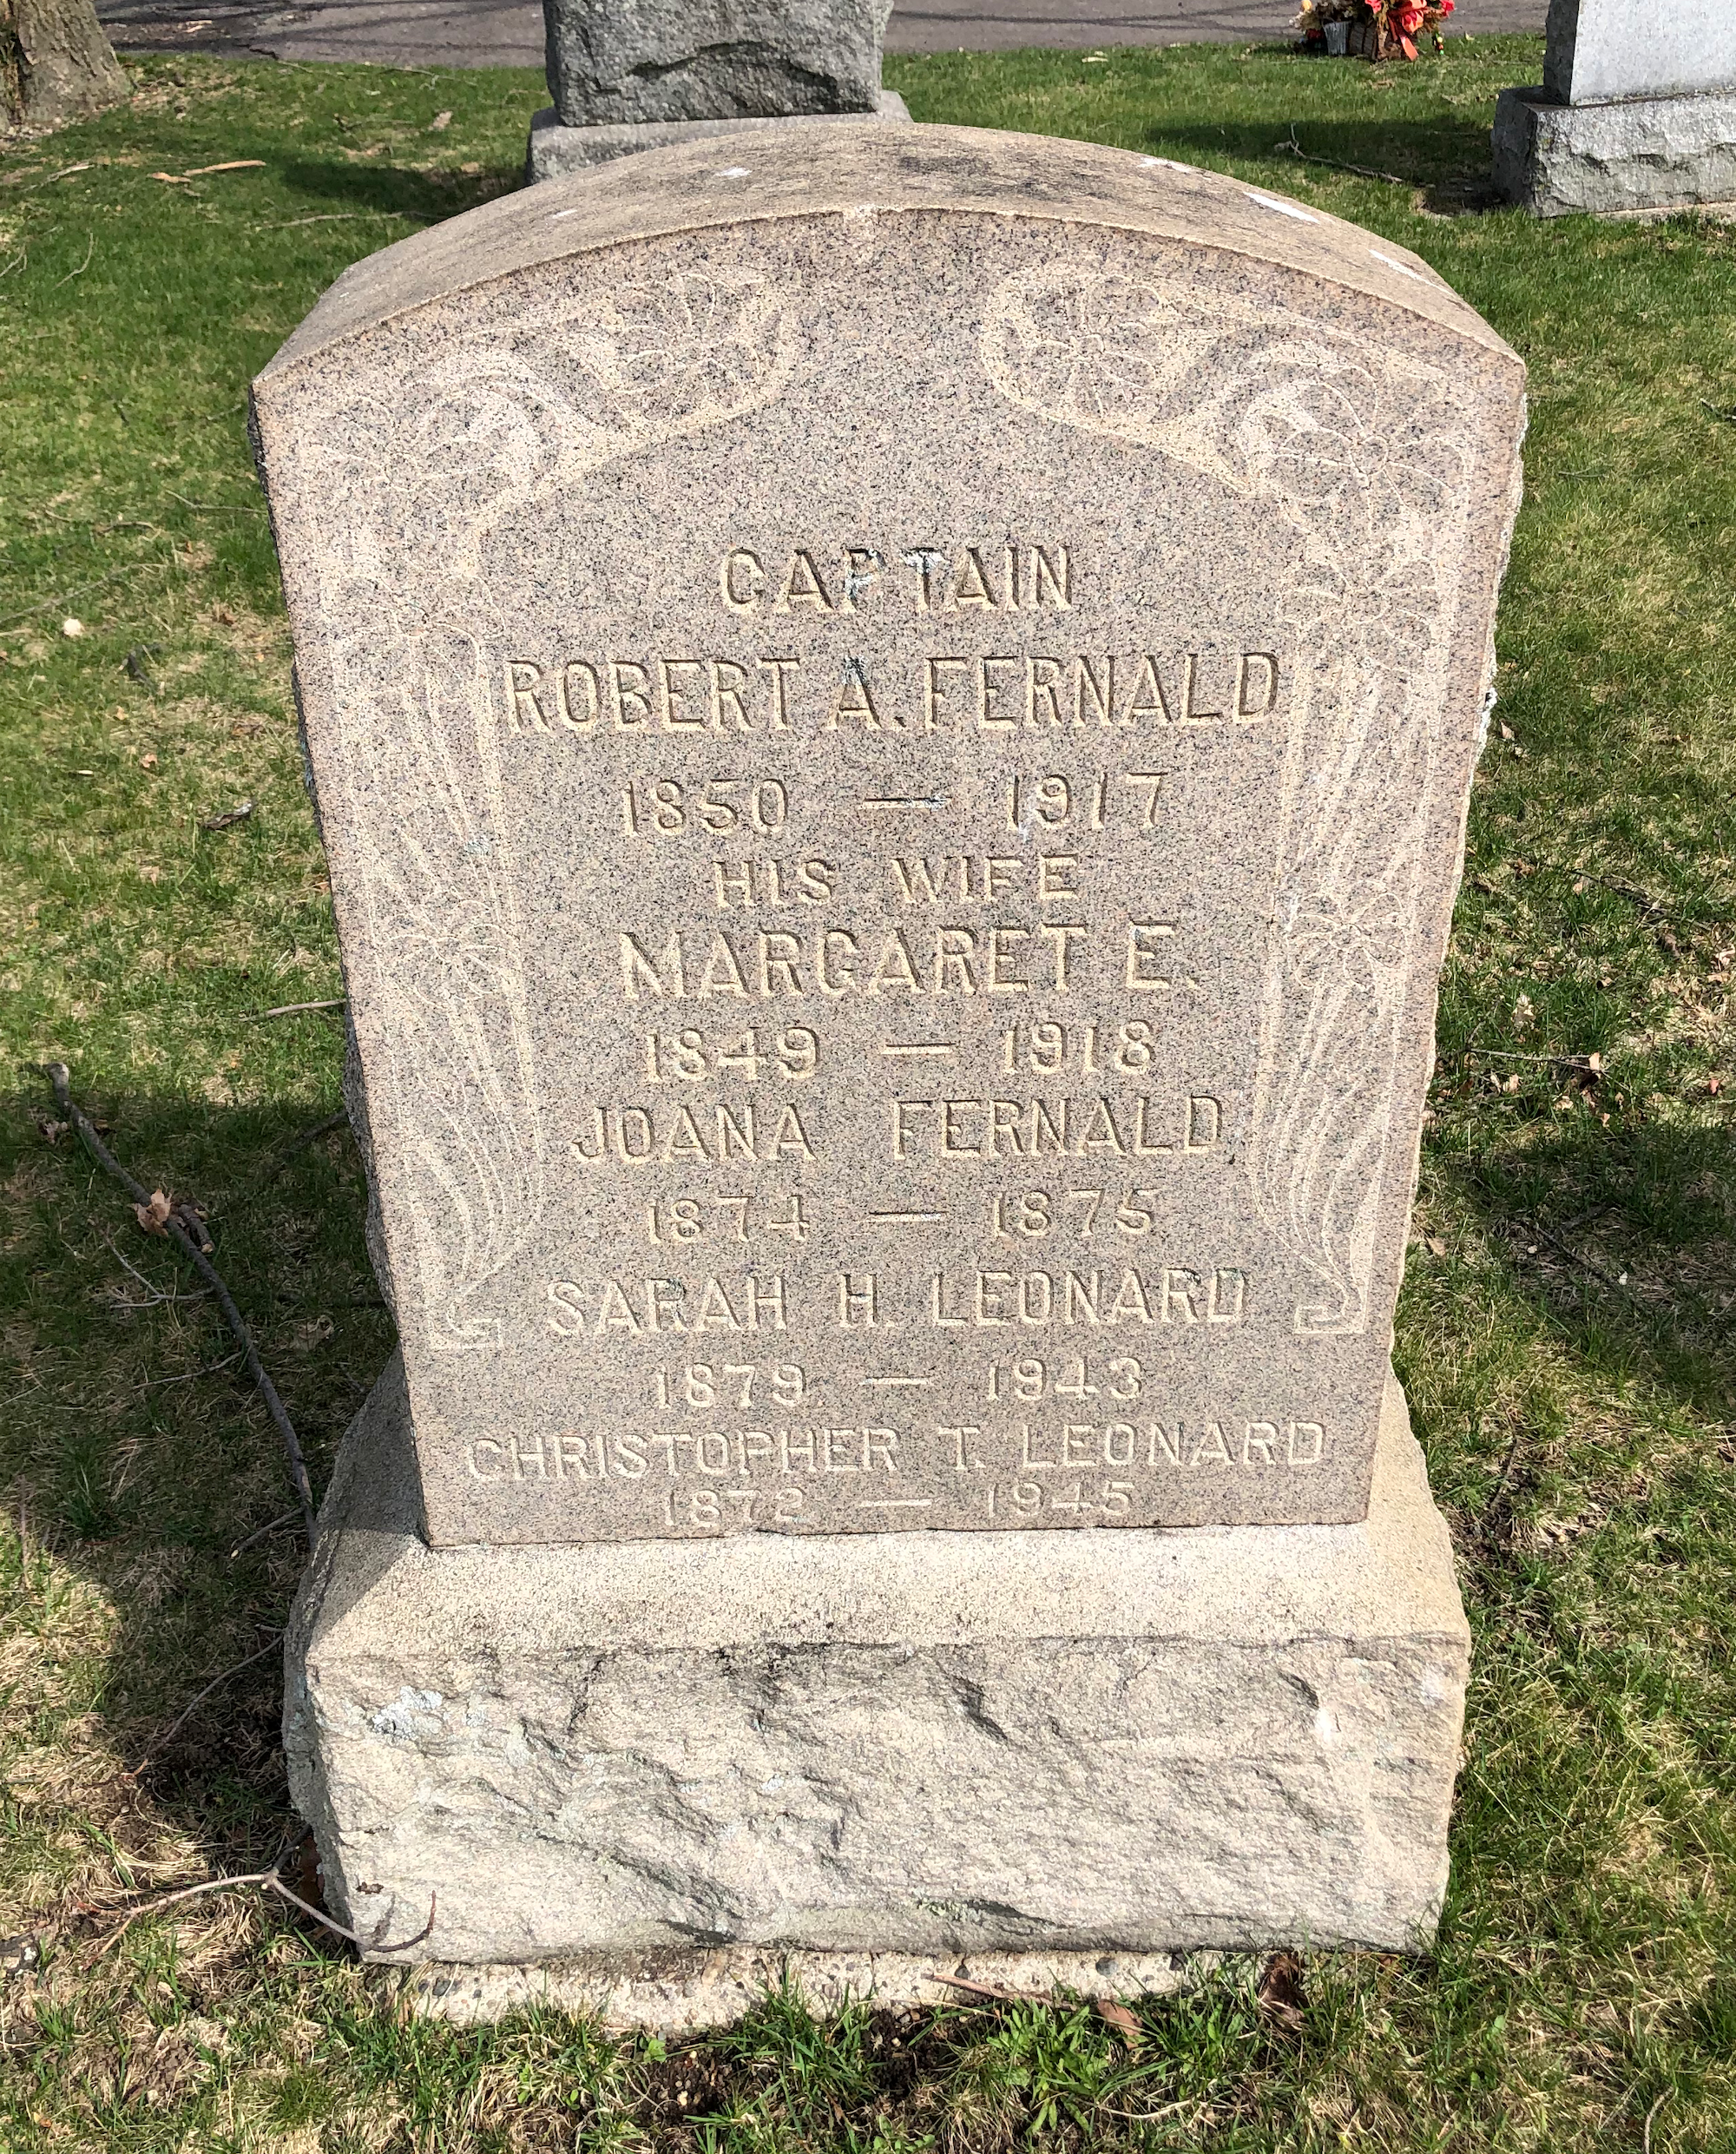
\includegraphics[width=\textwidth]{fernald_grave}
	\caption{Robert Fernald's family plot at Holy Cross Cemetery, Malden, Middlesex County, Massachusetts.\index{Holy Cross Cemetery}\index{Massachusetts!Malden} Photo by Gavin O'Brien, 14 April 2019.}
\end{figure}

\begin{table}[ht]
	\centering
	\caption{Holy Cross Cemetery\index{Holy Cross Cemetery}\cite{HolyCrossPlotFernald} \\
		Malden, Middlesex County, Massachusetts\index{Massachusetts!Malden}
		12 North Monument Path, Graves 37, 38 \& 2 Rear East}
	\begin{tabular}{|l|l|l|}
		\hline
		\textbf{Grave} & \textbf{Name} & \textbf{Burial Date} \\
		\hline
		37-Rear & Annie Fernald\index{Fernald!Anna\textsuperscript{4}} & 7 May 1875 \\ \hline
		37-Rear & John F. McCarthy\index{McCarthy!John F.\textsuperscript{5}} & 9 Oct 1881 \\ \hline
		38-Rear & Jeremiah Cooney\index{Cooney!Jeremiah} & 20 May 1883 \\ \hline
		37-Rear & William McCarthy\index{McCarthy!William\textsuperscript{5}} & 12 Jul 1885 \\ \hline
		37-Rear & Catherine McCarthy [Simonds]\index{Simonds!Catharine\textsuperscript{4}}\index{McCarthy!Catharine\textsuperscript{4} (Simonds)} & 27 Feb 1890 \\ \hline
		38 & Abrigain Dooley [Abigail O'Brien]\index{O'Brien!Abigail\textsuperscript{2}}\index{Dooley!Abigail\textsuperscript{2} (O'Brien)} & 6 Jan 1897 \\ \hline
		38-Rear & Hanna Cusick [Dooley]\index{Dooley!Hannah/Hanora\textsuperscript{3}}\index{Cooney!Hannah/Hanora\textsuperscript{3} (Dooley)}\index{Cusick!Hannah/Hanora\textsuperscript{3} (Dooley) (Cooney)} & 16 Jun 1911 \\ \hline
		37 & Robert W.\ Fernald [Robert A.\ Fernald]\index{Fernald!Robert} & 16 Jun 1917 \\ \hline
		37 & Margaret E. Fernald [Dooley]\index{Dooley!Margaret\textsuperscript{3}}\index{Fernald!Margaret\textsuperscript{3} (Dooley) (Simonds)}\index{Simonds!Margaret\textsuperscript{3} (Dooley)} & 4 Mar 1918 \\ \hline
		37-Rear & Caroline McGurin\index{McGurin!Caroline Josephine\textsuperscript{5}} & 5 Apr 1921 \\ \hline
		37-Rear & Josephine McGurin\index{McGurin!Josephine\textsuperscript{5}} & 22 May 1926 \\ \hline
		38-Rear & Caroline E. McGurin [Fernald]\index{Fernald!Caroline Emma\textsuperscript{4}}\index{McGurin!Caroline Emma\textsuperscript{4} (Fernald)} & 31 Aug 1927 \\ \hline
		37 & Sarah Leonard [Fernald]\index{Fernald!Sarah Helen\textsuperscript{4}}\index{Leonard!Sarah Helen\textsuperscript{4} (Fernald)} & 27 Mar 1943 \\ \hline
		38 & Christopher T.\ Leonard\index{Leonard!Christopher T.} & 12 Sep 1945 \\ \hline
		38-Rear & John J.\ McGurin\index{McGurin!John Joseph} & 13 Jan 1968 \\ \hline
		37 & Edward Joseph Duffy\index{Duffy!Edward J.} & 13 Apr 1983 \\ \hline
		38 & Mary M. Duffy [Leonard]\index{Leonard!Mary Margaret\textsuperscript{5}}\index{Duffy!Mary Margaret\textsuperscript{5} (Leonard)} & 3 Jun 1993 \\ \hline
	\end{tabular}
\end{table}

\begin{table}[ht]
	\centering
	\caption{Catholic Mt.\ Auburn Cemetery\index{Catholic Mt.\ Auburn Cemetery}\cite{BillMcEvoy} \\
		Watertown, Middlesex County, Massachusetts\index{Massachusetts!Watertown}
		Lot 103, Row 2 West (no marker)}
	\begin{tabular}{|l|l|}
		\hline
		\textbf{Name} & \textbf{Burial Date} \\
		\hline
		John O'Brien\index{O'Brien!John\textsuperscript{2}} & 26 Apr 1863 \\
		\hline
		Margaret O'Brien\index{O'Brien!Margaret\textsuperscript{3} (1862--1863)} & 25 Oct 1863 \\
		\hline
		Anna O'Brien\index{O'Brien!Anna\textsuperscript{3}} & 03 Mar 1866 \\
		\hline
		Bridget O'Brien [Colbert]\index{Colbert!Bridget}\index{O'Brien!Bridget (Colbert)} & 21 Oct 1873 \\
		\hline
		James E.\ O'Brien\index{O'Brien!James Edward\textsuperscript{3}} & 12 Apr 1879 \\
		\hline
		Ellen F.\ O'Brien\index{O'Brien!Ellen/Nellie\textsuperscript{3} (1859--1882)} & 01 Oct 1882 \\
		\hline
		Mary O'Brien\index{O'Brien!Mary\textsuperscript{3} (1856--1883)} & 18 Mar 1883 \\
		\hline
		Mary Bowser [Mahoney]\index{Mahoney/Mahony!Mary}\index{O'Brien!Mary (Mahoney)}\index{Bowser!Mary (Mahoney) (O'Brien)} & 18 Nov 1894 \\
		\hline
		Thomas J.\ Bowser\index{Bowser!Thomas} & 27 Mar 1903 \\
		\hline
	\end{tabular}
\end{table}

\begin{table}[ht]
	\centering
	\caption{Mt. Calvary Cemetery\index{Mt.\ Calvary Cemetery}\cite{John3OBrienBurial} \\
		Boston (Roslindale), Suffolk County, Massachusetts\index{Massachusetts!Boston!Roslindale}
		CL1-1 (Half Circle)}
	\begin{tabular}{|l|l|l|}
		\hline
		\textbf{Grave} & \textbf{Name} & \textbf{Burial Date} \\
		\hline
		1A & Catherine J.\ Mahoney [Kenney]\index{Kenney!Catherine Josephine}\index{Mahoney/Mahony!Catherine Josephine (Kenney)} & 13 Mar 1913 \\
		\hline
		1B & Elizabeth F.\ Mahoney\index{Mahoney/Mahony!Elizabeth F.} & 06 Jan 1936 \\
		\hline
		2A & Edward J.\ Mahoney\index{Mahoney/Mahony!Edward} & 15 Jul 1895 \\
		\hline
		2B & Almira L.\ Mahoney\index{Mahoney/Mahony!Almira L.} & 19 May 1910 \\
		\hline
		3A & Agnes P.\ Garvin\index{Garvin!Agnes P.} & 18 Aug 1883 \\
		\hline
		3B & William E.\ Garvin\index{Garvin!William E.} & 25 Oct 1886 \\
		\hline
		3C & Mary A.\ Garvin\index{Garvin!Mary A.} & 12 Jan 1916 \\
		\hline
		4A & Josephine L.\ Mahoney\index{Mahoney/Mahony!Josephine L.} & 17 May 1948 \\
		\hline
		5A & Pauline M.\ Baine [O'Brien]\index{O'Brien!Pauline M.\textsuperscript{4}}\index{Baine!Pauline M.\textsuperscript{4} (O'Brien)} & 04 Feb 1967 \\
		\hline
		6A & Mildred L.\ O'Brien\index{O'Brien!Mildred Loretta\textsuperscript{4}} & 26 May 1891 \\
		\hline
		6B & Edward O'Brien\index{O'Brien!Edward\textsuperscript{4} (1898--1898)} & 26 Dec 1898 \\
		\hline
		6C & Almira O'Brien\index{O'Brien!Almyra Louise\textsuperscript{4}} & 13 Jul 1902 \\
		\hline
		6D & John J.\ O'Brien\index{O'Brien!John Joseph\textsuperscript{3} (1861--1938)} & 17 May 1938 \\
		\hline
		6E & Emma A.\ O'Brien [Mahoney]\index{Mahoney/Mahony!Emma}\index{O'Brien!Emma (Mahony)} & 13 Jul 1950 \\
		\hline
	\end{tabular}
\end{table}

\begin{figure}
	\centering
	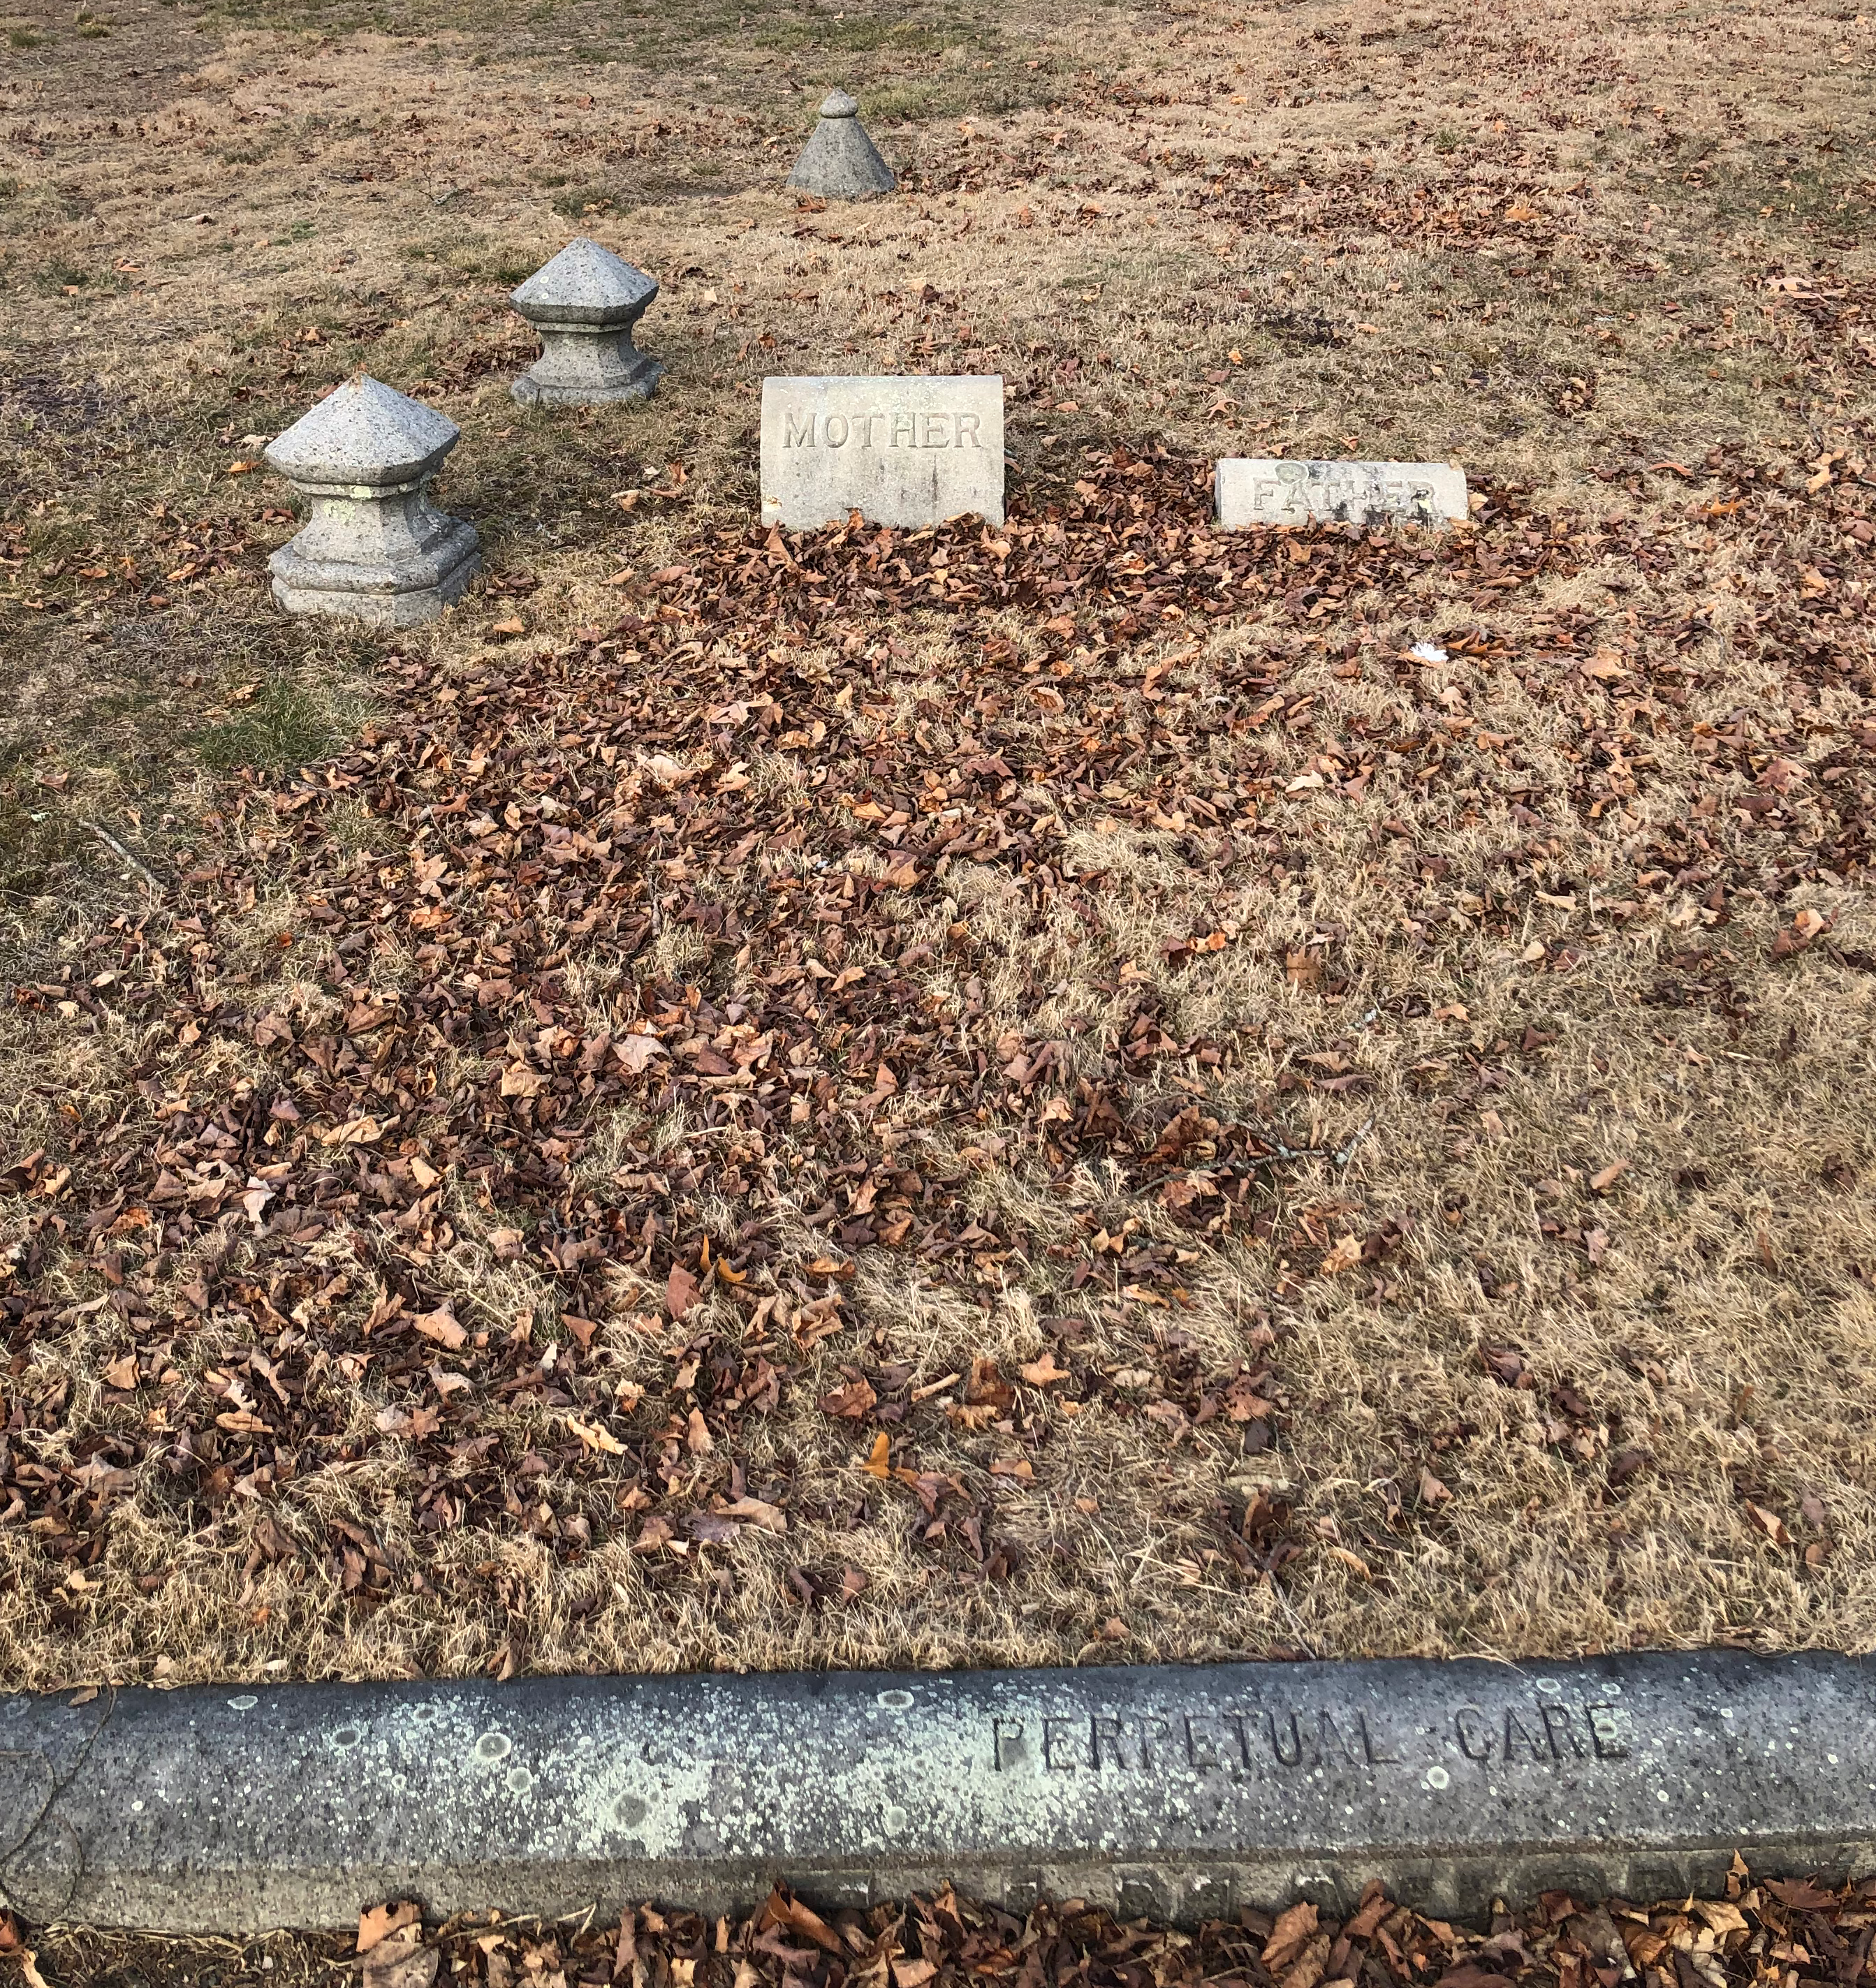
\includegraphics[width=\textwidth]{john_obrien_grave}
	\caption{Mahoney/Mahony family plot,\index{Mahoney/Mahony!family} Mt.\ Calvary Cemetery, Boston (Roslindale), Suffolk County, Massachusetts.\index{Massachusetts!Boston!Roslindale} Photo by Gavin O'Brien, 19 January 2021.}
\end{figure}

\begin{table}[ht]
	\centering
	\caption{Mt.\ Calvary Cemetery\index{Mt.\ Calvary Cemetery}\cite{William3OBrienBurial} \\
		Boston (Roslindale), Suffolk County, Massachusetts\index{Massachusetts!Boston!Roslindale}
		C7-22-22}
	\begin{tabular}{|l|l|}
		\hline
		\textbf{Name} & \textbf{Burial Date} \\
		\hline
		Julia T.\ O'Brien [McCarty]\index{McCarty!Julia T.}\index{O'Brien!Julia T.\ (McCarty)} & 11 Dec 1888 \\
		\hline
		William O'Brien\index{O'Brien!William\textsuperscript{3}} & 29 Oct 1889 \\
		\hline
		Nellie L.\ O'Brien\index{O'Brien!Ellen/Nellie Louise\textsuperscript{4}} & 15 Jun 1926 \\
		\hline
	\end{tabular}
\end{table}

\begin{figure}
	\centering
	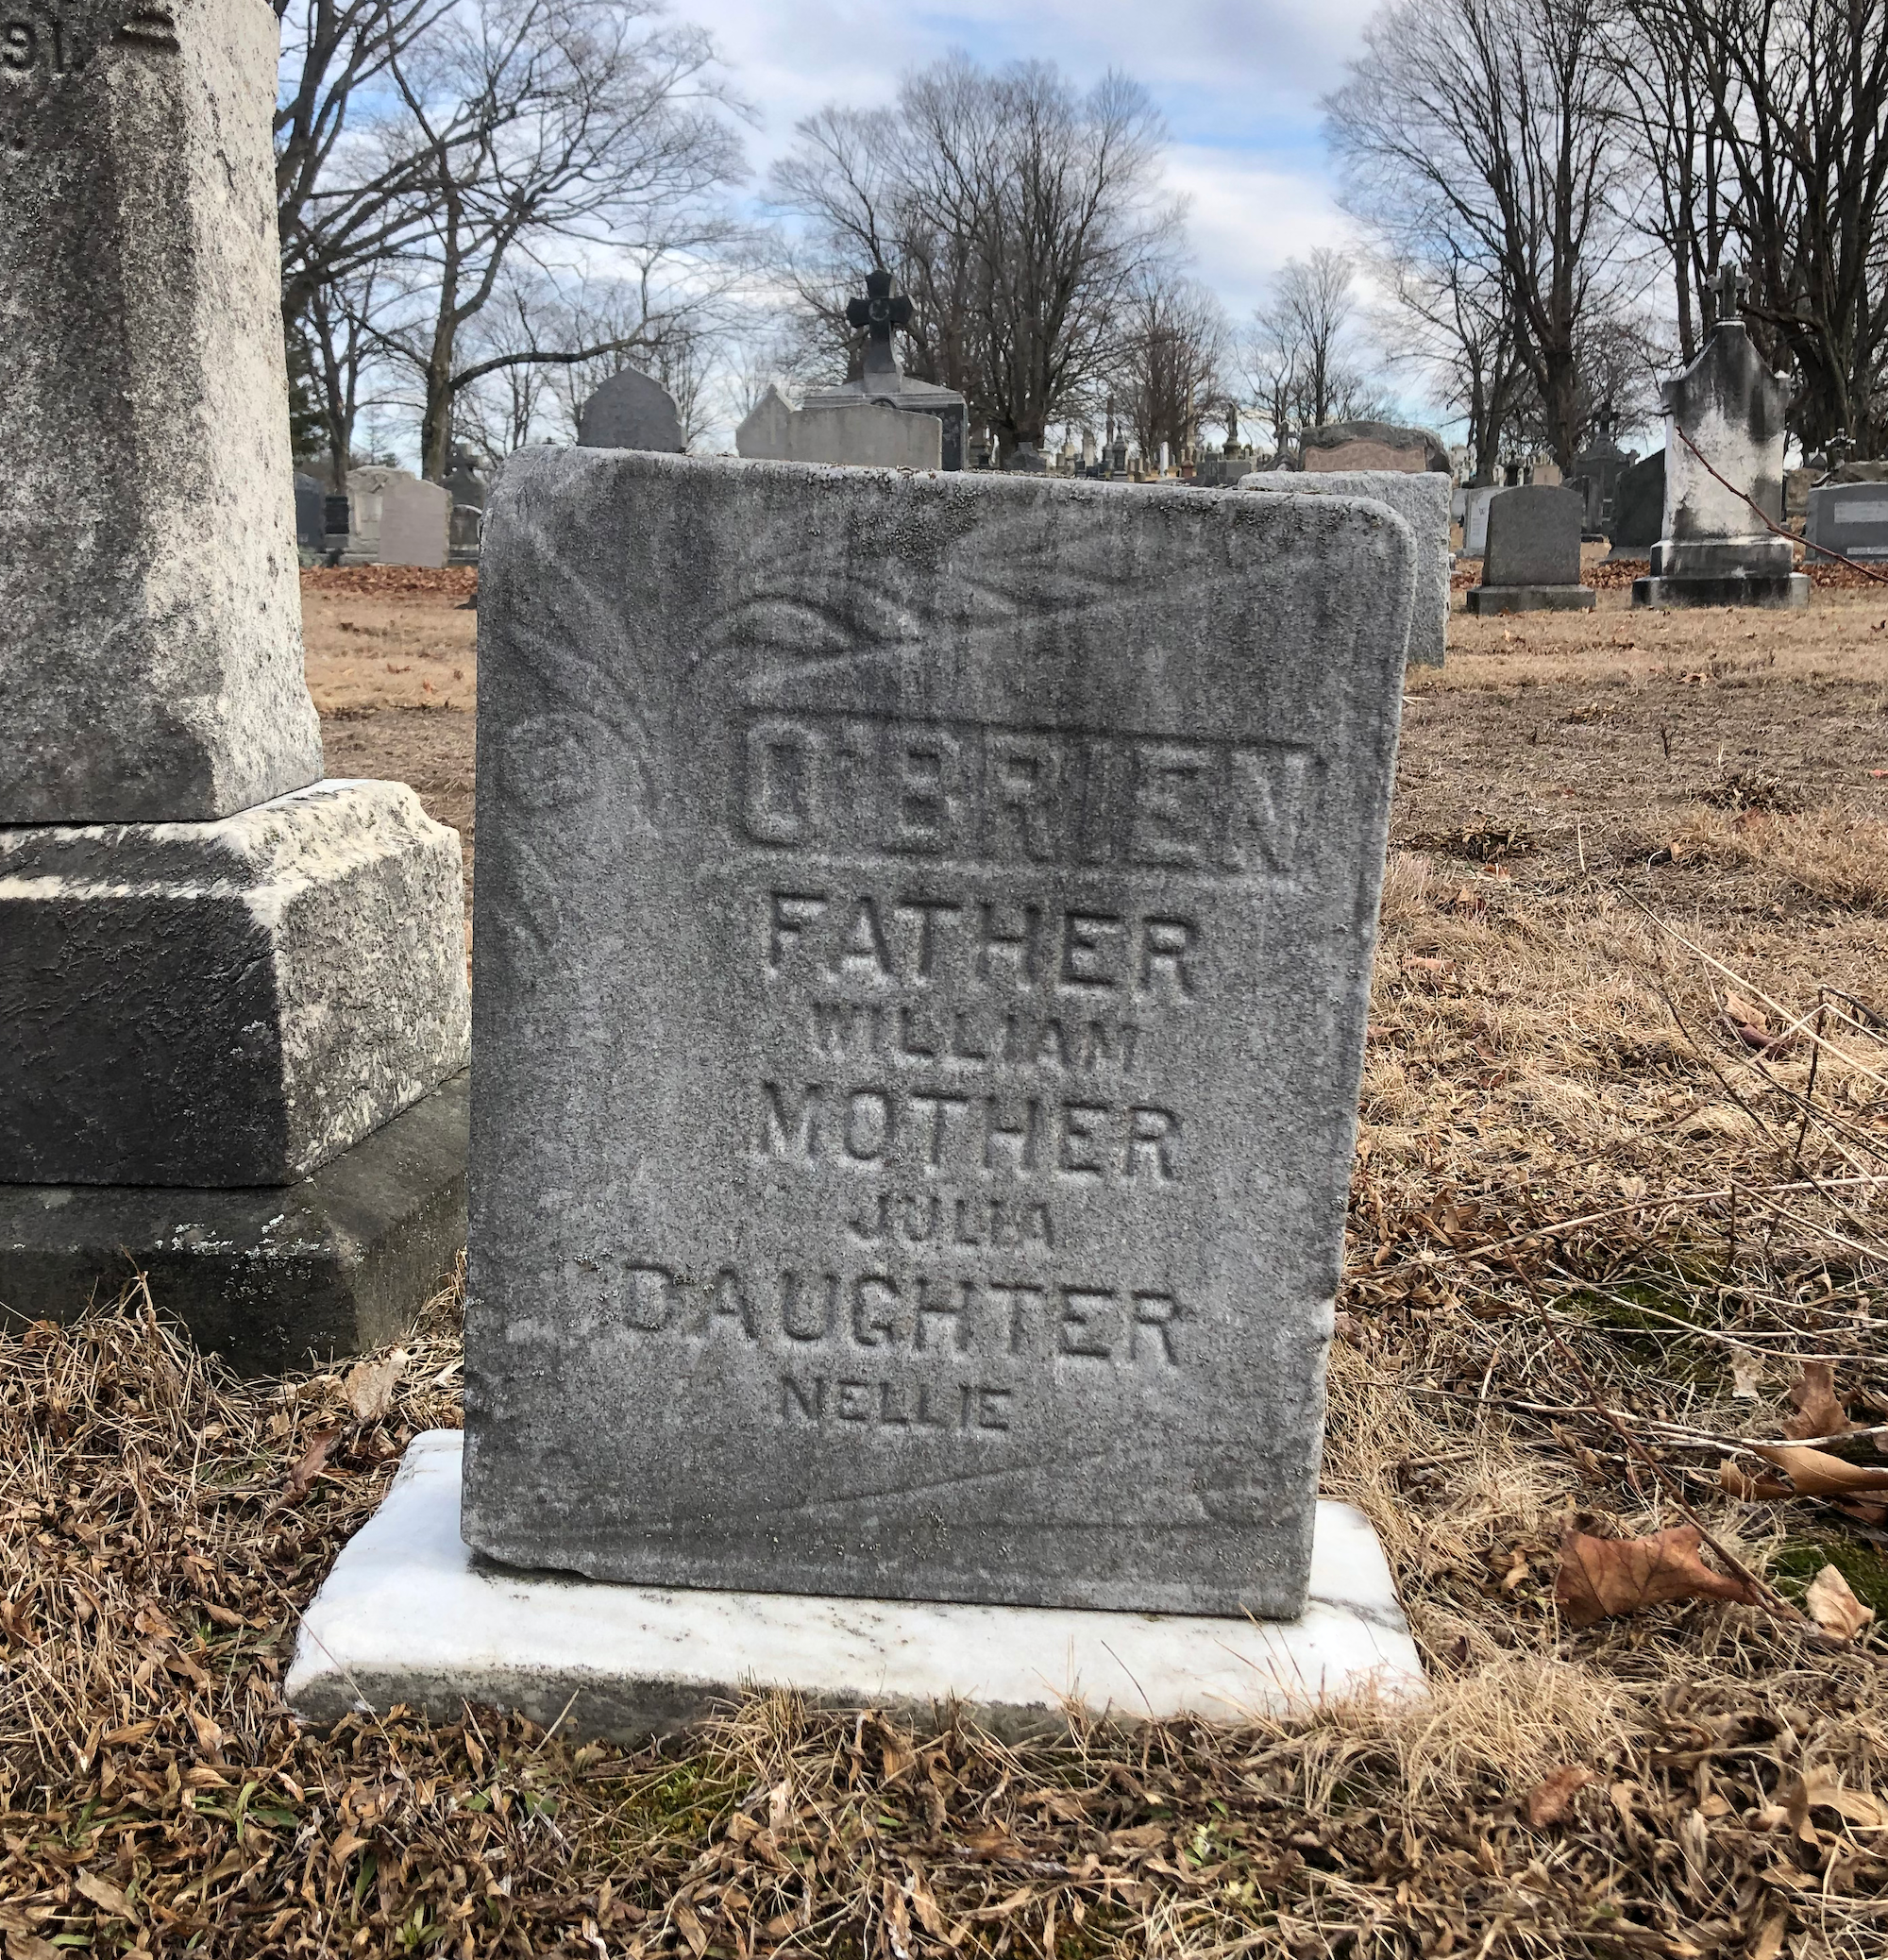
\includegraphics[width=\textwidth]{william_obrien_grave}
	\caption{William O'Brien\index{O'Brien!William\string\textsuperscript{2}} grave, Mt.\ Calvary Cemetery,\index{Mt.\ Calvary Cemetery} Boston (Roslindale), Suffolk County, Massachusetts.\index{Massachusetts!Boston!Roslindale} Photo by Gavin O'Brien, 19 Jan 2021.}
\end{figure}
